\documentclass{standalone}
\usepackage{tikz}
\usetikzlibrary{patterns, positioning}

\begin{document}
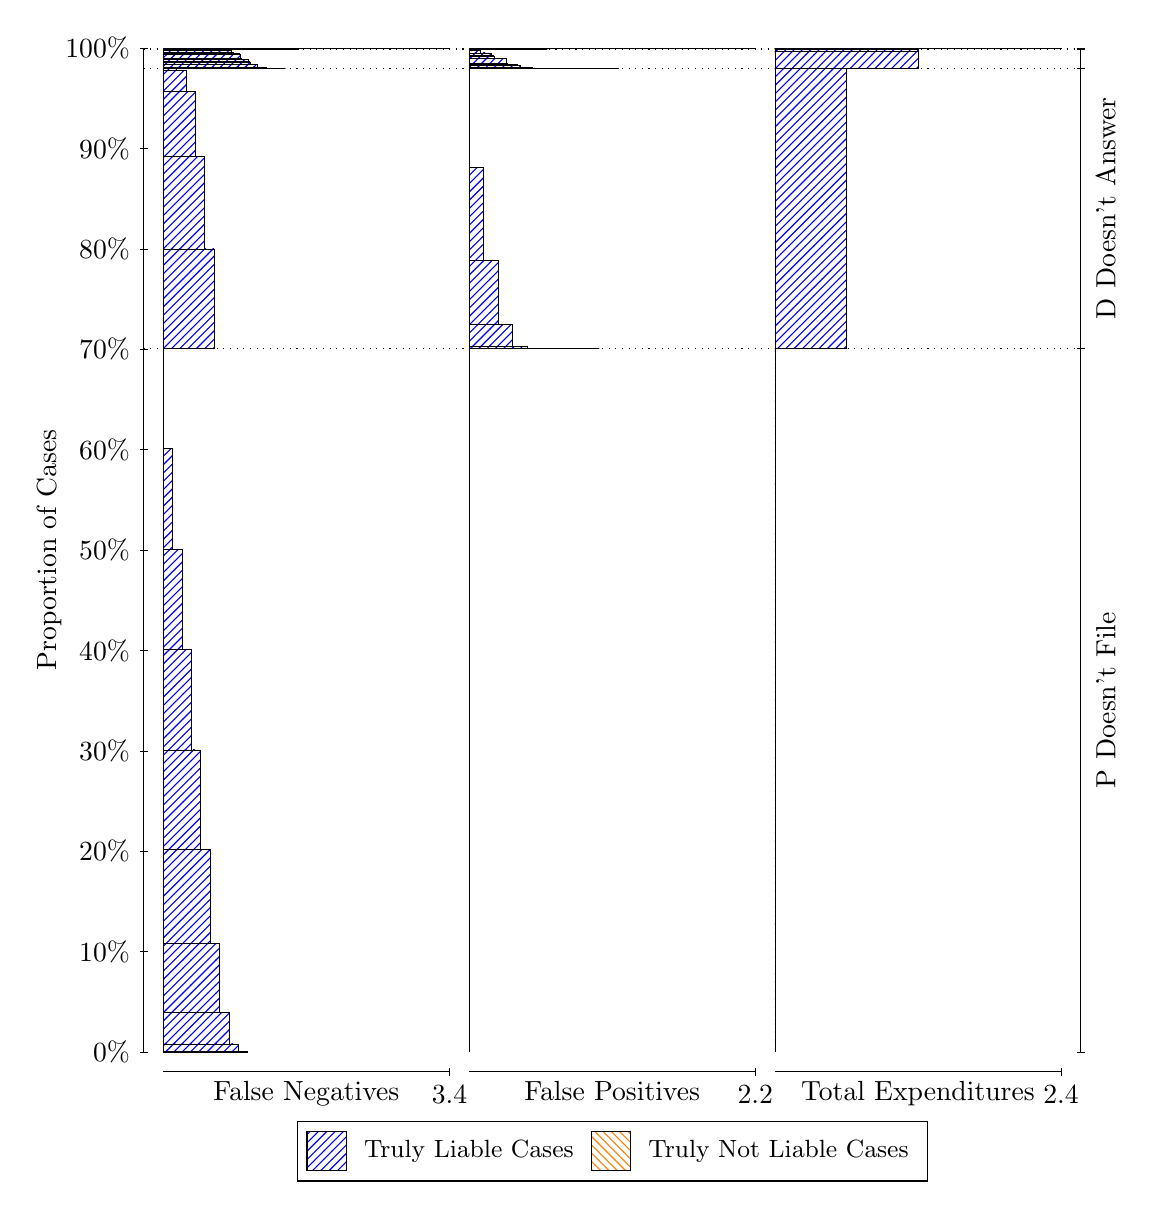
\begin{tikzpicture}
\draw[black, very thin] (1.5,1.75) -- (1.5,14.5);
\node[rotate=90, anchor=center] at (0.3, 8.125) {Proportion of Cases};
\draw[black, very thin] (1.45,1.75) -- (1.55,1.75);
\node[anchor=east] at (1.45, 1.75) {0\%};
\draw[black, very thin] (1.45,3.025) -- (1.55,3.025);
\node[anchor=east] at (1.45, 3.025) {10\%};
\draw[black, very thin] (1.45,4.3) -- (1.55,4.3);
\node[anchor=east] at (1.45, 4.3) {20\%};
\draw[black, very thin] (1.45,5.575) -- (1.55,5.575);
\node[anchor=east] at (1.45, 5.575) {30\%};
\draw[black, very thin] (1.45,6.85) -- (1.55,6.85);
\node[anchor=east] at (1.45, 6.85) {40\%};
\draw[black, very thin] (1.45,8.125) -- (1.55,8.125);
\node[anchor=east] at (1.45, 8.125) {50\%};
\draw[black, very thin] (1.45,9.4) -- (1.55,9.4);
\node[anchor=east] at (1.45, 9.4) {60\%};
\draw[black, very thin] (1.45,10.675) -- (1.55,10.675);
\node[anchor=east] at (1.45, 10.675) {70\%};
\draw[black, very thin] (1.45,11.95) -- (1.55,11.95);
\node[anchor=east] at (1.45, 11.95) {80\%};
\draw[black, very thin] (1.45,13.225) -- (1.55,13.225);
\node[anchor=east] at (1.45, 13.225) {90\%};
\draw[black, very thin] (1.45,14.5) -- (1.55,14.5);
\node[anchor=east] at (1.45, 14.5) {100\%};

\draw[black, very thin] (13.4,1.75) -- (13.4,14.5);
\draw[black, very thin] (13.35,1.75) -- (13.45,1.75);
\node[anchor=west] at (13.35, 1.75) {};
\draw[black, very thin] (13.35,10.687) -- (13.45,10.687);
\node[anchor=west] at (13.35, 10.687) {};
\draw[black, very thin] (13.35,14.245) -- (13.45,14.245);
\node[anchor=west] at (13.35, 14.245) {};
\draw[black, very thin] (13.35,14.482) -- (13.45,14.482);
\node[anchor=west] at (13.35, 14.482) {};
\draw[black, very thin] (13.35,14.495) -- (13.45,14.495);
\node[anchor=west] at (13.35, 14.495) {};
\draw[black, very thin] (13.35,14.496) -- (13.45,14.496);
\node[anchor=west] at (13.35, 14.496) {};
\draw[black, very thin] (13.35,14.5) -- (13.45,14.5);
\node[anchor=west] at (13.35, 14.5) {};

\draw[black, very thin, pattern color=blue, pattern=north east lines] (1.75,1.75) rectangle (2.8186,1.7615);
\draw[black, very thin, pattern color=blue, pattern=north east lines] (1.75,1.7615) rectangle (2.6999,1.8527);
\draw[black, very thin, pattern color=blue, pattern=north east lines] (1.75,1.8527) rectangle (2.5812,2.2486);
\draw[black, very thin, pattern color=blue, pattern=north east lines] (1.75,2.2486) rectangle (2.4624,3.1304);
\draw[black, very thin, pattern color=blue, pattern=north east lines] (1.75,3.1304) rectangle (2.3437,4.3202);
\draw[black, very thin, pattern color=blue, pattern=north east lines] (1.75,4.3202) rectangle (2.2249,5.5873);
\draw[black, very thin, pattern color=blue, pattern=north east lines] (1.75,5.5873) rectangle (2.1062,6.862);
\draw[black, very thin, pattern color=blue, pattern=north east lines] (1.75,6.862) rectangle (1.9875,8.137);
\draw[black, very thin, pattern color=blue, pattern=north east lines] (1.75,8.137) rectangle (1.8687,9.412);
\draw[black, very thin, pattern color=orange, pattern=north west lines] (1.75,9.412) rectangle (1.75,9.412);
\draw[black, very thin, pattern color=blue, pattern=north east lines] (1.75,9.412) rectangle (1.75,10.687);
\draw[black, very thin, pattern color=blue, pattern=north east lines] (1.75,10.687) rectangle (2.3912,11.95);
\draw[black, very thin, pattern color=blue, pattern=north east lines] (1.75,11.95) rectangle (2.2724,13.126);
\draw[black, very thin, pattern color=blue, pattern=north east lines] (1.75,13.126) rectangle (2.1537,13.946);
\draw[black, very thin, pattern color=blue, pattern=north east lines] (1.75,13.946) rectangle (2.035,14.218);
\draw[black, very thin, pattern color=blue, pattern=north east lines] (1.75,14.218) rectangle (1.9162,14.244);
\draw[black, very thin, pattern color=blue, pattern=north east lines] (1.75,14.244) rectangle (1.7975,14.245);
\draw[black, very thin, pattern color=orange, pattern=north west lines] (1.75,14.245) rectangle (1.75,14.245);
\draw[black, very thin, pattern color=blue, pattern=north east lines] (1.75,14.245) rectangle (1.75,14.245);
\draw[black, very thin, pattern color=blue, pattern=north east lines] (1.75,14.245) rectangle (3.2995,14.245);
\draw[black, very thin, pattern color=blue, pattern=north east lines] (1.75,14.245) rectangle (3.1926,14.245);
\draw[black, very thin, pattern color=blue, pattern=north east lines] (1.75,14.245) rectangle (3.1808,14.245);
\draw[black, very thin, pattern color=blue, pattern=north east lines] (1.75,14.245) rectangle (3.0858,14.245);
\draw[black, very thin, pattern color=blue, pattern=north east lines] (1.75,14.245) rectangle (3.0739,14.246);
\draw[black, very thin, pattern color=blue, pattern=north east lines] (1.75,14.246) rectangle (3.062,14.253);
\draw[black, very thin, pattern color=blue, pattern=north east lines] (1.75,14.253) rectangle (2.9789,14.253);
\draw[black, very thin, pattern color=blue, pattern=north east lines] (1.75,14.253) rectangle (2.967,14.255);
\draw[black, very thin, pattern color=blue, pattern=north east lines] (1.75,14.255) rectangle (2.9552,14.26);
\draw[black, very thin, pattern color=blue, pattern=north east lines] (1.75,14.26) rectangle (2.9433,14.29);
\draw[black, very thin, pattern color=blue, pattern=north east lines] (1.75,14.29) rectangle (2.8721,14.291);
\draw[black, very thin, pattern color=blue, pattern=north east lines] (1.75,14.291) rectangle (2.8602,14.292);
\draw[black, very thin, pattern color=blue, pattern=north east lines] (1.75,14.292) rectangle (2.8483,14.318);
\draw[black, very thin, pattern color=blue, pattern=north east lines] (1.75,14.318) rectangle (2.8364,14.328);
\draw[black, very thin, pattern color=blue, pattern=north east lines] (1.75,14.328) rectangle (2.8246,14.356);
\draw[black, very thin, pattern color=blue, pattern=north east lines] (1.75,14.356) rectangle (2.7533,14.359);
\draw[black, very thin, pattern color=blue, pattern=north east lines] (1.75,14.359) rectangle (2.7414,14.364);
\draw[black, very thin, pattern color=blue, pattern=north east lines] (1.75,14.364) rectangle (2.7296,14.364);
\draw[black, very thin, pattern color=blue, pattern=north east lines] (1.75,14.364) rectangle (2.7296,14.424);
\draw[black, very thin, pattern color=blue, pattern=north east lines] (1.75,14.424) rectangle (2.7177,14.428);
\draw[black, very thin, pattern color=blue, pattern=north east lines] (1.75,14.428) rectangle (2.7058,14.433);
\draw[black, very thin, pattern color=blue, pattern=north east lines] (1.75,14.433) rectangle (2.6346,14.443);
\draw[black, very thin, pattern color=blue, pattern=north east lines] (1.75,14.443) rectangle (2.6227,14.448);
\draw[black, very thin, pattern color=blue, pattern=north east lines] (1.75,14.448) rectangle (2.6108,14.471);
\draw[black, very thin, pattern color=blue, pattern=north east lines] (1.75,14.471) rectangle (2.599,14.471);
\draw[black, very thin, pattern color=blue, pattern=north east lines] (1.75,14.471) rectangle (2.5871,14.471);
\draw[black, very thin, pattern color=blue, pattern=north east lines] (1.75,14.471) rectangle (2.5158,14.479);
\draw[black, very thin, pattern color=blue, pattern=north east lines] (1.75,14.479) rectangle (2.504,14.48);
\draw[black, very thin, pattern color=blue, pattern=north east lines] (1.75,14.48) rectangle (2.4921,14.481);
\draw[black, very thin, pattern color=blue, pattern=north east lines] (1.75,14.481) rectangle (2.4802,14.481);
\draw[black, very thin, pattern color=blue, pattern=north east lines] (1.75,14.481) rectangle (2.4684,14.481);
\draw[black, very thin, pattern color=blue, pattern=north east lines] (1.75,14.481) rectangle (2.3971,14.482);
\draw[black, very thin, pattern color=blue, pattern=north east lines] (1.75,14.482) rectangle (2.3852,14.482);
\draw[black, very thin, pattern color=blue, pattern=north east lines] (1.75,14.482) rectangle (2.3734,14.482);
\draw[black, very thin, pattern color=blue, pattern=north east lines] (1.75,14.482) rectangle (2.3615,14.482);
\draw[black, very thin, pattern color=blue, pattern=north east lines] (1.75,14.482) rectangle (2.3496,14.482);
\draw[black, very thin, pattern color=blue, pattern=north east lines] (1.75,14.482) rectangle (2.2784,14.482);
\draw[black, very thin, pattern color=blue, pattern=north east lines] (1.75,14.482) rectangle (2.2665,14.482);
\draw[black, very thin, pattern color=blue, pattern=north east lines] (1.75,14.482) rectangle (2.2546,14.482);
\draw[black, very thin, pattern color=blue, pattern=north east lines] (1.75,14.482) rectangle (2.2546,14.482);
\draw[black, very thin, pattern color=blue, pattern=north east lines] (1.75,14.482) rectangle (2.2428,14.482);
\draw[black, very thin, pattern color=blue, pattern=north east lines] (1.75,14.482) rectangle (2.2309,14.482);
\draw[black, very thin, pattern color=blue, pattern=north east lines] (1.75,14.482) rectangle (2.1596,14.482);
\draw[black, very thin, pattern color=blue, pattern=north east lines] (1.75,14.482) rectangle (2.1478,14.482);
\draw[black, very thin, pattern color=blue, pattern=north east lines] (1.75,14.482) rectangle (2.1359,14.482);
\draw[black, very thin, pattern color=blue, pattern=north east lines] (1.75,14.482) rectangle (2.1359,14.482);
\draw[black, very thin, pattern color=blue, pattern=north east lines] (1.75,14.482) rectangle (2.124,14.482);
\draw[black, very thin, pattern color=blue, pattern=north east lines] (1.75,14.482) rectangle (2.0409,14.482);
\draw[black, very thin, pattern color=blue, pattern=north east lines] (1.75,14.482) rectangle (2.029,14.482);
\draw[black, very thin, pattern color=blue, pattern=north east lines] (1.75,14.482) rectangle (2.0172,14.482);
\draw[black, very thin, pattern color=blue, pattern=north east lines] (1.75,14.482) rectangle (2.0172,14.482);
\draw[black, very thin, pattern color=blue, pattern=north east lines] (1.75,14.482) rectangle (1.9222,14.482);
\draw[black, very thin, pattern color=blue, pattern=north east lines] (1.75,14.482) rectangle (1.9103,14.482);
\draw[black, very thin, pattern color=blue, pattern=north east lines] (1.75,14.482) rectangle (1.8034,14.482);
\draw[black, very thin, pattern color=orange, pattern=north west lines] (1.75,14.482) rectangle (1.75,14.482);
\draw[black, very thin, pattern color=blue, pattern=north east lines] (1.75,14.482) rectangle (3.4598,14.483);
\draw[black, very thin, pattern color=blue, pattern=north east lines] (1.75,14.483) rectangle (3.3411,14.483);
\draw[black, very thin, pattern color=blue, pattern=north east lines] (1.75,14.483) rectangle (3.2223,14.487);
\draw[black, very thin, pattern color=blue, pattern=north east lines] (1.75,14.487) rectangle (3.1036,14.493);
\draw[black, very thin, pattern color=blue, pattern=north east lines] (1.75,14.493) rectangle (2.9849,14.495);
\draw[black, very thin, pattern color=blue, pattern=north east lines] (1.75,14.495) rectangle (2.8661,14.495);
\draw[black, very thin, pattern color=blue, pattern=north east lines] (1.75,14.495) rectangle (2.7474,14.495);
\draw[black, very thin, pattern color=blue, pattern=north east lines] (1.75,14.495) rectangle (2.6286,14.495);
\draw[black, very thin, pattern color=blue, pattern=north east lines] (1.75,14.495) rectangle (2.5099,14.495);
\draw[black, very thin, pattern color=blue, pattern=north east lines] (1.75,14.495) rectangle (2.3912,14.495);
\draw[black, very thin, pattern color=orange, pattern=north west lines] (1.75,14.495) rectangle (1.75,14.495);
\draw[black, very thin, pattern color=blue, pattern=north east lines] (1.75,14.495) rectangle (2.3912,14.495);
\draw[black, very thin, pattern color=blue, pattern=north east lines] (1.75,14.495) rectangle (2.2724,14.495);
\draw[black, very thin, pattern color=blue, pattern=north east lines] (1.75,14.495) rectangle (2.1537,14.496);
\draw[black, very thin, pattern color=blue, pattern=north east lines] (1.75,14.496) rectangle (2.035,14.496);
\draw[black, very thin, pattern color=blue, pattern=north east lines] (1.75,14.496) rectangle (1.9162,14.496);
\draw[black, very thin, pattern color=blue, pattern=north east lines] (1.75,14.496) rectangle (1.7975,14.496);
\draw[black, very thin, pattern color=orange, pattern=north west lines] (1.75,14.496) rectangle (1.75,14.496);
\draw[black, very thin, pattern color=blue, pattern=north east lines] (1.75,14.496) rectangle (1.75,14.496);
\draw[black, very thin, pattern color=blue, pattern=north east lines] (1.75,14.496) rectangle (5.3833,14.496);
\draw[black, very thin, pattern color=blue, pattern=north east lines] (1.75,14.496) rectangle (5.2646,14.496);
\draw[black, very thin, pattern color=blue, pattern=north east lines] (1.75,14.496) rectangle (5.1459,14.496);
\draw[black, very thin, pattern color=blue, pattern=north east lines] (1.75,14.496) rectangle (5.0271,14.496);
\draw[black, very thin, pattern color=blue, pattern=north east lines] (1.75,14.496) rectangle (4.9084,14.496);
\draw[black, very thin, pattern color=blue, pattern=north east lines] (1.75,14.496) rectangle (4.9084,14.496);
\draw[black, very thin, pattern color=blue, pattern=north east lines] (1.75,14.496) rectangle (4.7897,14.496);
\draw[black, very thin, pattern color=blue, pattern=north east lines] (1.75,14.496) rectangle (4.6709,14.496);
\draw[black, very thin, pattern color=blue, pattern=north east lines] (1.75,14.496) rectangle (4.6709,14.496);
\draw[black, very thin, pattern color=blue, pattern=north east lines] (1.75,14.496) rectangle (4.5522,14.496);
\draw[black, very thin, pattern color=blue, pattern=north east lines] (1.75,14.496) rectangle (4.5522,14.496);
\draw[black, very thin, pattern color=blue, pattern=north east lines] (1.75,14.496) rectangle (4.4334,14.496);
\draw[black, very thin, pattern color=blue, pattern=north east lines] (1.75,14.496) rectangle (4.3147,14.496);
\draw[black, very thin, pattern color=blue, pattern=north east lines] (1.75,14.496) rectangle (4.196,14.496);
\draw[black, very thin, pattern color=blue, pattern=north east lines] (1.75,14.496) rectangle (4.0772,14.496);
\draw[black, very thin, pattern color=blue, pattern=north east lines] (1.75,14.496) rectangle (3.9585,14.496);
\draw[black, very thin, pattern color=blue, pattern=north east lines] (1.75,14.496) rectangle (3.8635,14.496);
\draw[black, very thin, pattern color=blue, pattern=north east lines] (1.75,14.496) rectangle (3.7448,14.496);
\draw[black, very thin, pattern color=blue, pattern=north east lines] (1.75,14.496) rectangle (3.626,14.496);
\draw[black, very thin, pattern color=blue, pattern=north east lines] (1.75,14.496) rectangle (3.5073,14.496);
\draw[black, very thin, pattern color=blue, pattern=north east lines] (1.75,14.496) rectangle (3.3886,14.496);
\draw[black, very thin, pattern color=blue, pattern=north east lines] (1.75,14.496) rectangle (3.2698,14.496);
\draw[black, very thin, pattern color=blue, pattern=north east lines] (1.75,14.496) rectangle (3.2698,14.497);
\draw[black, very thin, pattern color=blue, pattern=north east lines] (1.75,14.497) rectangle (3.1511,14.497);
\draw[black, very thin, pattern color=blue, pattern=north east lines] (1.75,14.497) rectangle (3.1511,14.498);
\draw[black, very thin, pattern color=blue, pattern=north east lines] (1.75,14.498) rectangle (3.0324,14.499);
\draw[black, very thin, pattern color=blue, pattern=north east lines] (1.75,14.499) rectangle (2.9136,14.499);
\draw[black, very thin, pattern color=blue, pattern=north east lines] (1.75,14.499) rectangle (2.9136,14.5);
\draw[black, very thin, pattern color=blue, pattern=north east lines] (1.75,14.5) rectangle (2.7949,14.5);
\draw[black, very thin, pattern color=blue, pattern=north east lines] (1.75,14.5) rectangle (2.7949,14.5);
\draw[black, very thin, pattern color=blue, pattern=north east lines] (1.75,14.5) rectangle (2.7949,14.5);
\draw[black, very thin, pattern color=blue, pattern=north east lines] (1.75,14.5) rectangle (2.6761,14.5);
\draw[black, very thin, pattern color=blue, pattern=north east lines] (1.75,14.5) rectangle (2.6761,14.5);
\draw[black, very thin, pattern color=blue, pattern=north east lines] (1.75,14.5) rectangle (2.5574,14.5);
\draw[black, very thin, pattern color=blue, pattern=north east lines] (1.75,14.5) rectangle (2.4387,14.5);
\draw[black, very thin, pattern color=blue, pattern=north east lines] (1.75,14.5) rectangle (2.3199,14.5);
\draw[black, very thin, pattern color=blue, pattern=north east lines] (1.75,14.5) rectangle (2.3199,14.5);
\draw[black, very thin, pattern color=blue, pattern=north east lines] (1.75,14.5) rectangle (2.2012,14.5);
\draw[black, very thin, pattern color=blue, pattern=north east lines] (1.75,14.5) rectangle (2.2012,14.5);
\draw[black, very thin, pattern color=blue, pattern=north east lines] (1.75,14.5) rectangle (2.0825,14.5);
\draw[black, very thin, pattern color=blue, pattern=north east lines] (1.75,14.5) rectangle (2.0825,14.5);
\draw[black, very thin, pattern color=blue, pattern=north east lines] (1.75,14.5) rectangle (1.9637,14.5);
\draw[black, very thin, pattern color=orange, pattern=north west lines] (1.75,14.5) rectangle (1.75,14.5);
\draw[black, very thin, pattern color=orange, pattern=north west lines] (5.6333,1.75) rectangle (5.6333,1.75);
\draw[black, very thin, pattern color=blue, pattern=north east lines] (5.6333,1.75) rectangle (5.6333,10.687);
\draw[black, very thin, pattern color=orange, pattern=north west lines] (5.6333,10.687) rectangle (7.2848,10.687);
\draw[black, very thin, pattern color=blue, pattern=north east lines] (5.6333,10.687) rectangle (7.2848,10.687);
\draw[black, very thin, pattern color=blue, pattern=north east lines] (5.6333,10.687) rectangle (7.1013,10.687);
\draw[black, very thin, pattern color=blue, pattern=north east lines] (5.6333,10.687) rectangle (6.9178,10.687);
\draw[black, very thin, pattern color=blue, pattern=north east lines] (5.6333,10.687) rectangle (6.7343,10.687);
\draw[black, very thin, pattern color=blue, pattern=north east lines] (5.6333,10.687) rectangle (6.5508,10.688);
\draw[black, very thin, pattern color=blue, pattern=north east lines] (5.6333,10.688) rectangle (6.3673,10.714);
\draw[black, very thin, pattern color=blue, pattern=north east lines] (5.6333,10.714) rectangle (6.1838,10.986);
\draw[black, very thin, pattern color=blue, pattern=north east lines] (5.6333,10.986) rectangle (6.0003,11.806);
\draw[black, very thin, pattern color=blue, pattern=north east lines] (5.6333,11.806) rectangle (5.8168,12.982);
\draw[black, very thin, pattern color=blue, pattern=north east lines] (5.6333,12.982) rectangle (5.6333,14.245);
\draw[black, very thin, pattern color=orange, pattern=north west lines] (5.6333,14.245) rectangle (7.5326,14.245);
\draw[black, very thin, pattern color=blue, pattern=north east lines] (5.6333,14.245) rectangle (7.5326,14.245);
\draw[black, very thin, pattern color=orange, pattern=north west lines] (5.6333,14.245) rectangle (7.3674,14.245);
\draw[black, very thin, pattern color=blue, pattern=north east lines] (5.6333,14.245) rectangle (7.3674,14.245);
\draw[black, very thin, pattern color=blue, pattern=north east lines] (5.6333,14.245) rectangle (7.3491,14.245);
\draw[black, very thin, pattern color=orange, pattern=north west lines] (5.6333,14.245) rectangle (7.2023,14.245);
\draw[black, very thin, pattern color=blue, pattern=north east lines] (5.6333,14.245) rectangle (7.2023,14.245);
\draw[black, very thin, pattern color=blue, pattern=north east lines] (5.6333,14.245) rectangle (7.1839,14.245);
\draw[black, very thin, pattern color=blue, pattern=north east lines] (5.6333,14.245) rectangle (7.1656,14.245);
\draw[black, very thin, pattern color=orange, pattern=north west lines] (5.6333,14.245) rectangle (7.0371,14.245);
\draw[black, very thin, pattern color=blue, pattern=north east lines] (5.6333,14.245) rectangle (7.0371,14.245);
\draw[black, very thin, pattern color=blue, pattern=north east lines] (5.6333,14.245) rectangle (7.0188,14.245);
\draw[black, very thin, pattern color=blue, pattern=north east lines] (5.6333,14.245) rectangle (7.0004,14.245);
\draw[black, very thin, pattern color=blue, pattern=north east lines] (5.6333,14.245) rectangle (6.9821,14.245);
\draw[black, very thin, pattern color=orange, pattern=north west lines] (5.6333,14.245) rectangle (6.872,14.245);
\draw[black, very thin, pattern color=blue, pattern=north east lines] (5.6333,14.245) rectangle (6.872,14.245);
\draw[black, very thin, pattern color=blue, pattern=north east lines] (5.6333,14.245) rectangle (6.8536,14.245);
\draw[black, very thin, pattern color=blue, pattern=north east lines] (5.6333,14.245) rectangle (6.8353,14.245);
\draw[black, very thin, pattern color=blue, pattern=north east lines] (5.6333,14.245) rectangle (6.8169,14.245);
\draw[black, very thin, pattern color=blue, pattern=north east lines] (5.6333,14.245) rectangle (6.7986,14.245);
\draw[black, very thin, pattern color=blue, pattern=north east lines] (5.6333,14.245) rectangle (6.6885,14.245);
\draw[black, very thin, pattern color=blue, pattern=north east lines] (5.6333,14.245) rectangle (6.6701,14.245);
\draw[black, very thin, pattern color=blue, pattern=north east lines] (5.6333,14.245) rectangle (6.6518,14.245);
\draw[black, very thin, pattern color=blue, pattern=north east lines] (5.6333,14.245) rectangle (6.6334,14.245);
\draw[black, very thin, pattern color=blue, pattern=north east lines] (5.6333,14.245) rectangle (6.6151,14.246);
\draw[black, very thin, pattern color=blue, pattern=north east lines] (5.6333,14.246) rectangle (6.505,14.246);
\draw[black, very thin, pattern color=blue, pattern=north east lines] (5.6333,14.246) rectangle (6.4866,14.246);
\draw[black, very thin, pattern color=blue, pattern=north east lines] (5.6333,14.246) rectangle (6.4683,14.247);
\draw[black, very thin, pattern color=blue, pattern=north east lines] (5.6333,14.247) rectangle (6.4499,14.248);
\draw[black, very thin, pattern color=blue, pattern=north east lines] (5.6333,14.248) rectangle (6.4316,14.256);
\draw[black, very thin, pattern color=blue, pattern=north east lines] (5.6333,14.256) rectangle (6.3215,14.256);
\draw[black, very thin, pattern color=blue, pattern=north east lines] (5.6333,14.256) rectangle (6.3031,14.257);
\draw[black, very thin, pattern color=blue, pattern=north east lines] (5.6333,14.257) rectangle (6.2848,14.28);
\draw[black, very thin, pattern color=blue, pattern=north east lines] (5.6333,14.28) rectangle (6.2664,14.284);
\draw[black, very thin, pattern color=blue, pattern=north east lines] (5.6333,14.284) rectangle (6.2481,14.294);
\draw[black, very thin, pattern color=blue, pattern=north east lines] (5.6333,14.294) rectangle (6.138,14.299);
\draw[black, very thin, pattern color=blue, pattern=north east lines] (5.6333,14.299) rectangle (6.1196,14.303);
\draw[black, very thin, pattern color=blue, pattern=north east lines] (5.6333,14.303) rectangle (6.1013,14.364);
\draw[black, very thin, pattern color=blue, pattern=north east lines] (5.6333,14.364) rectangle (6.0829,14.368);
\draw[black, very thin, pattern color=blue, pattern=north east lines] (5.6333,14.368) rectangle (6.0646,14.371);
\draw[black, very thin, pattern color=blue, pattern=north east lines] (5.6333,14.371) rectangle (5.9545,14.399);
\draw[black, very thin, pattern color=blue, pattern=north east lines] (5.6333,14.399) rectangle (5.9361,14.409);
\draw[black, very thin, pattern color=blue, pattern=north east lines] (5.6333,14.409) rectangle (5.9178,14.436);
\draw[black, very thin, pattern color=blue, pattern=north east lines] (5.6333,14.436) rectangle (5.8994,14.437);
\draw[black, very thin, pattern color=blue, pattern=north east lines] (5.6333,14.437) rectangle (5.8811,14.437);
\draw[black, very thin, pattern color=blue, pattern=north east lines] (5.6333,14.437) rectangle (5.771,14.467);
\draw[black, very thin, pattern color=blue, pattern=north east lines] (5.6333,14.467) rectangle (5.7526,14.472);
\draw[black, very thin, pattern color=blue, pattern=north east lines] (5.6333,14.472) rectangle (5.7343,14.474);
\draw[black, very thin, pattern color=blue, pattern=north east lines] (5.6333,14.474) rectangle (5.7159,14.474);
\draw[black, very thin, pattern color=blue, pattern=north east lines] (5.6333,14.474) rectangle (5.6333,14.482);
\draw[black, very thin, pattern color=orange, pattern=north west lines] (5.6333,14.482) rectangle (6.6242,14.482);
\draw[black, very thin, pattern color=blue, pattern=north east lines] (5.6333,14.482) rectangle (6.6242,14.482);
\draw[black, very thin, pattern color=blue, pattern=north east lines] (5.6333,14.482) rectangle (6.4407,14.482);
\draw[black, very thin, pattern color=blue, pattern=north east lines] (5.6333,14.482) rectangle (6.2572,14.482);
\draw[black, very thin, pattern color=blue, pattern=north east lines] (5.6333,14.482) rectangle (6.0737,14.483);
\draw[black, very thin, pattern color=blue, pattern=north east lines] (5.6333,14.483) rectangle (5.8902,14.483);
\draw[black, very thin, pattern color=blue, pattern=north east lines] (5.6333,14.483) rectangle (5.7067,14.485);
\draw[black, very thin, pattern color=blue, pattern=north east lines] (5.6333,14.485) rectangle (5.6333,14.495);
\draw[black, very thin, pattern color=orange, pattern=north west lines] (5.6333,14.495) rectangle (8.2758,14.495);
\draw[black, very thin, pattern color=blue, pattern=north east lines] (5.6333,14.495) rectangle (8.2758,14.495);
\draw[black, very thin, pattern color=blue, pattern=north east lines] (5.6333,14.495) rectangle (8.0923,14.495);
\draw[black, very thin, pattern color=blue, pattern=north east lines] (5.6333,14.495) rectangle (7.9088,14.495);
\draw[black, very thin, pattern color=blue, pattern=north east lines] (5.6333,14.495) rectangle (7.7253,14.495);
\draw[black, very thin, pattern color=blue, pattern=north east lines] (5.6333,14.495) rectangle (7.5418,14.495);
\draw[black, very thin, pattern color=blue, pattern=north east lines] (5.6333,14.495) rectangle (7.3582,14.495);
\draw[black, very thin, pattern color=blue, pattern=north east lines] (5.6333,14.495) rectangle (7.1747,14.496);
\draw[black, very thin, pattern color=blue, pattern=north east lines] (5.6333,14.496) rectangle (6.9912,14.496);
\draw[black, very thin, pattern color=blue, pattern=north east lines] (5.6333,14.496) rectangle (6.8077,14.496);
\draw[black, very thin, pattern color=blue, pattern=north east lines] (5.6333,14.496) rectangle (6.6242,14.496);
\draw[black, very thin, pattern color=orange, pattern=north west lines] (5.6333,14.496) rectangle (9.2667,14.496);
\draw[black, very thin, pattern color=blue, pattern=north east lines] (5.6333,14.496) rectangle (9.2667,14.496);
\draw[black, very thin, pattern color=blue, pattern=north east lines] (5.6333,14.496) rectangle (9.0832,14.496);
\draw[black, very thin, pattern color=orange, pattern=north west lines] (5.6333,14.496) rectangle (9.0832,14.496);
\draw[black, very thin, pattern color=blue, pattern=north east lines] (5.6333,14.496) rectangle (9.0832,14.496);
\draw[black, very thin, pattern color=orange, pattern=north west lines] (5.6333,14.496) rectangle (8.8997,14.496);
\draw[black, very thin, pattern color=blue, pattern=north east lines] (5.6333,14.496) rectangle (8.8997,14.496);
\draw[black, very thin, pattern color=blue, pattern=north east lines] (5.6333,14.496) rectangle (8.8997,14.496);
\draw[black, very thin, pattern color=blue, pattern=north east lines] (5.6333,14.496) rectangle (8.7162,14.496);
\draw[black, very thin, pattern color=orange, pattern=north west lines] (5.6333,14.496) rectangle (8.7162,14.496);
\draw[black, very thin, pattern color=blue, pattern=north east lines] (5.6333,14.496) rectangle (8.7162,14.496);
\draw[black, very thin, pattern color=blue, pattern=north east lines] (5.6333,14.496) rectangle (8.7162,14.496);
\draw[black, very thin, pattern color=blue, pattern=north east lines] (5.6333,14.496) rectangle (8.5327,14.496);
\draw[black, very thin, pattern color=orange, pattern=north west lines] (5.6333,14.496) rectangle (8.5327,14.496);
\draw[black, very thin, pattern color=blue, pattern=north east lines] (5.6333,14.496) rectangle (8.5327,14.496);
\draw[black, very thin, pattern color=blue, pattern=north east lines] (5.6333,14.496) rectangle (8.5327,14.496);
\draw[black, very thin, pattern color=blue, pattern=north east lines] (5.6333,14.496) rectangle (8.3492,14.496);
\draw[black, very thin, pattern color=orange, pattern=north west lines] (5.6333,14.496) rectangle (8.3492,14.496);
\draw[black, very thin, pattern color=blue, pattern=north east lines] (5.6333,14.496) rectangle (8.3492,14.496);
\draw[black, very thin, pattern color=blue, pattern=north east lines] (5.6333,14.496) rectangle (8.3492,14.496);
\draw[black, very thin, pattern color=blue, pattern=north east lines] (5.6333,14.496) rectangle (8.1657,14.496);
\draw[black, very thin, pattern color=blue, pattern=north east lines] (5.6333,14.496) rectangle (8.1657,14.496);
\draw[black, very thin, pattern color=orange, pattern=north west lines] (5.6333,14.496) rectangle (8.1657,14.496);
\draw[black, very thin, pattern color=blue, pattern=north east lines] (5.6333,14.496) rectangle (8.1657,14.496);
\draw[black, very thin, pattern color=blue, pattern=north east lines] (5.6333,14.496) rectangle (8.1657,14.496);
\draw[black, very thin, pattern color=blue, pattern=north east lines] (5.6333,14.496) rectangle (7.9822,14.496);
\draw[black, very thin, pattern color=blue, pattern=north east lines] (5.6333,14.496) rectangle (7.9822,14.496);
\draw[black, very thin, pattern color=orange, pattern=north west lines] (5.6333,14.496) rectangle (7.9822,14.496);
\draw[black, very thin, pattern color=blue, pattern=north east lines] (5.6333,14.496) rectangle (7.9822,14.496);
\draw[black, very thin, pattern color=blue, pattern=north east lines] (5.6333,14.496) rectangle (7.7987,14.497);
\draw[black, very thin, pattern color=blue, pattern=north east lines] (5.6333,14.497) rectangle (7.7987,14.497);
\draw[black, very thin, pattern color=blue, pattern=north east lines] (5.6333,14.497) rectangle (7.7987,14.497);
\draw[black, very thin, pattern color=blue, pattern=north east lines] (5.6333,14.497) rectangle (7.6152,14.498);
\draw[black, very thin, pattern color=blue, pattern=north east lines] (5.6333,14.498) rectangle (7.6152,14.498);
\draw[black, very thin, pattern color=blue, pattern=north east lines] (5.6333,14.498) rectangle (7.6152,14.498);
\draw[black, very thin, pattern color=blue, pattern=north east lines] (5.6333,14.498) rectangle (7.4316,14.499);
\draw[black, very thin, pattern color=blue, pattern=north east lines] (5.6333,14.499) rectangle (7.4316,14.499);
\draw[black, very thin, pattern color=blue, pattern=north east lines] (5.6333,14.499) rectangle (7.4316,14.499);
\draw[black, very thin, pattern color=blue, pattern=north east lines] (5.6333,14.499) rectangle (7.2481,14.499);
\draw[black, very thin, pattern color=blue, pattern=north east lines] (5.6333,14.499) rectangle (7.2481,14.5);
\draw[black, very thin, pattern color=blue, pattern=north east lines] (5.6333,14.5) rectangle (7.2481,14.5);
\draw[black, very thin, pattern color=blue, pattern=north east lines] (5.6333,14.5) rectangle (7.0646,14.5);
\draw[black, very thin, pattern color=blue, pattern=north east lines] (5.6333,14.5) rectangle (7.0646,14.5);
\draw[black, very thin, pattern color=blue, pattern=north east lines] (5.6333,14.5) rectangle (7.0646,14.5);
\draw[black, very thin, pattern color=blue, pattern=north east lines] (5.6333,14.5) rectangle (6.8811,14.5);
\draw[black, very thin, pattern color=blue, pattern=north east lines] (5.6333,14.5) rectangle (6.8811,14.5);
\draw[black, very thin, pattern color=blue, pattern=north east lines] (5.6333,14.5) rectangle (6.6976,14.5);
\draw[black, very thin, pattern color=blue, pattern=north east lines] (5.6333,14.5) rectangle (6.6976,14.5);
\draw[black, very thin, pattern color=blue, pattern=north east lines] (5.6333,14.5) rectangle (6.5141,14.5);
\draw[black, very thin, pattern color=blue, pattern=north east lines] (5.6333,14.5) rectangle (6.3306,14.5);
\draw[black, very thin, pattern color=orange, pattern=north west lines] (5.6333,14.5) rectangle (6.1838,14.5);
\draw[black, very thin, pattern color=blue, pattern=north east lines] (5.6333,14.5) rectangle (6.1838,14.5);
\draw[black, very thin, pattern color=orange, pattern=north west lines] (5.6333,14.5) rectangle (6.0003,14.5);
\draw[black, very thin, pattern color=blue, pattern=north east lines] (5.6333,14.5) rectangle (6.0003,14.5);
\draw[black, very thin, pattern color=orange, pattern=north west lines] (5.6333,14.5) rectangle (5.8168,14.5);
\draw[black, very thin, pattern color=blue, pattern=north east lines] (5.6333,14.5) rectangle (5.8168,14.5);
\draw[black, very thin, pattern color=orange, pattern=north west lines] (5.6333,14.5) rectangle (5.6333,14.5);
\draw[black, very thin, pattern color=blue, pattern=north east lines] (5.6333,14.5) rectangle (5.6333,14.5);
\draw[black, very thin, pattern color=orange, pattern=north west lines] (9.5167,1.75) rectangle (9.5167,1.75);
\draw[black, very thin, pattern color=blue, pattern=north east lines] (9.5167,1.75) rectangle (9.5167,10.687);
\draw[black, very thin, pattern color=orange, pattern=north west lines] (9.5167,10.687) rectangle (10.425,10.687);
\draw[black, very thin, pattern color=blue, pattern=north east lines] (9.5167,10.687) rectangle (10.425,14.245);
\draw[black, very thin, pattern color=orange, pattern=north west lines] (9.5167,14.245) rectangle (11.333,14.245);
\draw[black, very thin, pattern color=blue, pattern=north east lines] (9.5167,14.245) rectangle (11.333,14.46);
\draw[black, very thin, pattern color=orange, pattern=north west lines] (9.5167,14.46) rectangle (11.333,14.46);
\draw[black, very thin, pattern color=blue, pattern=north east lines] (9.5167,14.46) rectangle (11.333,14.482);
\draw[black, very thin, pattern color=orange, pattern=north west lines] (9.5167,14.482) rectangle (11.333,14.482);
\draw[black, very thin, pattern color=blue, pattern=north east lines] (9.5167,14.482) rectangle (11.333,14.495);
\draw[black, very thin, pattern color=orange, pattern=north west lines] (9.5167,14.495) rectangle (11.333,14.495);
\draw[black, very thin, pattern color=blue, pattern=north east lines] (9.5167,14.495) rectangle (11.333,14.496);
\draw[black, very thin, pattern color=orange, pattern=north west lines] (9.5167,14.496) rectangle (13.15,14.496);
\draw[black, very thin, pattern color=blue, pattern=north east lines] (9.5167,14.496) rectangle (13.15,14.496);
\draw[black, very thin, pattern color=orange, pattern=north west lines] (9.5167,14.496) rectangle (13.15,14.496);
\draw[black, very thin, pattern color=blue, pattern=north east lines] (9.5167,14.496) rectangle (13.15,14.499);
\draw[black, very thin, pattern color=orange, pattern=north west lines] (9.5167,14.499) rectangle (13.15,14.499);
\draw[black, very thin, pattern color=blue, pattern=north east lines] (9.5167,14.499) rectangle (13.15,14.5);
\draw[black, dotted] (1.5,10.687) -- (13.4,10.687);
\draw[black, dotted] (1.5,14.245) -- (13.4,14.245);
\draw[black, dotted] (1.5,14.482) -- (13.4,14.482);
\draw[black, dotted] (1.5,14.495) -- (13.4,14.495);
\draw[black, dotted] (1.5,14.496) -- (13.4,14.496);
\draw[black, very thin] (1.75,1.5) -- (5.3833,1.5);
\node[anchor=north] at (3.5667, 1.5) {False Negatives};
\draw[black, very thin] (5.3833,1.45) -- (5.3833,1.55);
\node[anchor=north] at (5.3833, 1.45) {3.4};

\draw[black, very thin] (5.6333,1.5) -- (9.2667,1.5);
\node[anchor=north] at (7.45, 1.5) {False Positives};
\draw[black, very thin] (9.2667,1.45) -- (9.2667,1.55);
\node[anchor=north] at (9.2667, 1.45) {2.2};

\draw[black, very thin] (9.5167,1.5) -- (13.15,1.5);
\node[anchor=north] at (11.333, 1.5) {Total Expenditures};
\draw[black, very thin] (13.15,1.45) -- (13.15,1.55);
\node[anchor=north] at (13.15, 1.45) {2.4};

\node[black, centered, rotate=90] at (13.72, 6.2185) {P Doesn't File};
\node[black, centered, rotate=90] at (13.72, 12.466) {D Doesn't Answer};





\draw (7.449999999999999,1.5) node[draw=none] (baseCoordinate) {};
\begin{scope}[align=center]
        \matrix[scale=0.5, draw=black, below=0.5cm of baseCoordinate, nodes={draw}, column sep=0.1cm]{
            \node[rectangle, draw, minimum width=0.5cm, minimum height=0.5cm, pattern=north east lines, pattern color=blue] {}; &
            \node[draw=none, font=\small] (B) {Truly Liable Cases}; &
            \node[rectangle, draw, minimum width=0.5cm, minimum height=0.5cm, pattern=north west lines, pattern color=orange] {}; &
            \node[draw=none, font=\small] (B) {Truly Not Liable Cases}; \\
            };
\end{scope}

\end{tikzpicture}
\end{document}